\documentclass{iopconfser}

\usepackage{float}
\usepackage{graphicx}
\usepackage{subcaption}
\usepackage{ragged2e}
\usepackage[export]{adjustbox}
\usepackage{mathtools}
\usepackage[automake]{glossaries-extra}


% \makeglossaries

\setabbreviationstyle[acronym]{long-postshort-user}
\glssetcategoryattribute{acronym}{nohyperfirst}{true}
\setabbreviationstyle{short-nolong}
\makeglossaries

% --------------------
% ---- Glossaries ----
% --------------------
\newglossaryentry{asyncio}{name=Asyncio, description={A Python library for asynchronous code.}}
\newglossaryentry{stim}{name=STIM300, description={A MEMS-based \gls{imu}}}
\newglossaryentry{f9p}{name=F9P, description={A Global Navigation Satellite System (GNSS) receiver manufactured by u-blox.}}

% --------------------
% ----- Acronyms -----
% --------------------
\newacronym{asv}{ASV}{Autonomous Surface Vehicle}
\newacronym{dolp}{DoLP}{Degree of Linear Polarization}
\newacronym{aolp}{AoLP}{Angle of Linear Polarization}
\newacronym{sitaw}{SITAW}{Situational Awareness}
\newacronym{poe}{PoE}{Power over Ethernet}
\newacronym{pps}{PPS}{Pulse Per Second}
\newacronym{cpfa}{CPFA}{Color-Polarization Filter Array}
\newacronym{utc}{UTC}{Coordinated Universal Time}
\newacronym{imu}{IMU}{Inertial Measurement Unit}
\newacronym{tov}{TOV}{Time of Validity}
\newacronym{tm2}{TM2}{Time mark data}
\newacronym{gnss}{GNSS}{Global Navigation Satellite System}
\newacronym{ptp}{PTP}{Precision Time Protocol}

% \glsaddall
% \makenoidxglossaries

% \glsunset{cpu}
\glsunset{gnss}
\glsunset{imu}
\glsunset{tm2}
\glsunset{utc}

% --------------------
% ----- Shortcuts ----
% --------------------


\addbibresource{mylib.bib}


\begin{document}

\title{A Lightweight, Polarization-Camera Equipped Sensor Rig for the Development of Autonomous Surface Vehicles}

\author{Emil Martens$^{1}$, Edmund Førland Brekke$^{1}$, Rudolf Mester$^{2}$, Annette Stahl$^{1}$}

\affil{$^1$Department of Engineering Cybernetics, NTNU, Trondheim, Norway}

\affil{$^2$Department of Computer Science, NTNU, Trondheim, Norway}

\email{emil.martens@ntnu.no}


\begin{abstract}
    \justifying
    \gls{sitaw} of \glspl{asv} is critical for safe and efficient maritime operations, enabling these vehicles to understand their environment better and make informed decisions.
    High-quality data sets from relevant maritime environments are needed to advance the development of \gls{sitaw}, as it is both the backbone of any learning-based method and the development and validation of classical methods.
    Research vessels such as the full-scale ferry \textit{milliAmpere2} provide such data, but there tends to be a considerable labor cost associated with their operation.
    With this in mind, we have developed a portable sensor rig that makes collecting sensor data significantly easier.
    
    The sensor rig is designed for easy transport and operation by a single individual. 
    It can also be temporarily attached to an existing vessel, making it versatile for a wide range of data collection scenarios.
    The sensor rig is equipped with a Jetson Orin AGX computer, two dual-band GNSS receivers, a high-quality IMU, and two color polarization cameras.
    Accurate synchronization of all sensors and the computer to \gls{utc} is achieved using a microcontroller for triggering and a custom PPS-enabled Linux kernel on the Jetson.
    The sensor rig is controlled and monitored by connecting a smartphone to its hosted web app, which provides a live stream from the cameras and information about the sensors.
    
    We present a new dataset from the river Nidelva in Trondheim, Norway, to demonstrate the sensor rig's potential and the benefit of color polarization cameras in the maritime domain.
    We show how the data from color polarization cameras can be used directly to make the water surface more visibly distinct and remove reflections and sun glare.
    This new data set consists of synchronized stereo color polarization video, raw IMU data, and raw GNSS data, and it is made publically available to the research community.
    
\end{abstract}

\pagebreak

\section{Introduction}
\glspl{asv} have received attention in recent years and several vessels have been built for research, such as \textit{Milliampere}, \textit{Milliampere 2}, and \textit{Maverick} \cite{brekkeMilliAmpereAutonomousFerry2022}\cite{zhangDesignBuildAutonomous2023}\cite{eideAutonomousUrbanPassenger2024}.
To operate autonomously, these vehicles are all equipped with multiple sensors to perceive their environment, achieve \gls{sitaw}, and make informed decisions.
The choice of sensors plays a crucial role in the design, development, and operation of \glspl{asv}, and there is a wide range of types and models to pick from on the market \cite{thombreSensorsAITechniques2022}.
To make informed decisions about what sensors to use and advance the development of \glspl{asv}, it is therefore important to have access to data collected from various combinations of sensors in relevant maritime environments.

The data collected from research vessels are valuable for this purpose and necessary for many types of research.
Unfortunately, collecting data this way generally involves multiple people and depends on the \gls{asv} being operational, which is not always the case.
Varying the types and placement of sensors on the vessels and calibrating them is also generally impractical.
To make this easier, we have designed and developed a lightweight sensor rig to be carried and operated by a single person or temporarily attached to an existing vessel \cite{martensPavingWayEnhanced2023}.
It is not intended as a replacement for research vessels but rather as a complement for any research group working on \gls{sitaw} for \glspl{asv} to augment the data collection capabilities.
With the development of the sensor rig, we decided to use the opportunity to explore the potential of color polarization cameras in the maritime domain, which were not mentioned in the otherwise comprehensive review of sensors for \gls{sitaw} by Thombre et al. \cite{thombreSensorsAITechniques2022}.
Research on the use of polarization cameras in the maritime domain for target recognition and image dehazing has been published \cite{zhongPolarizationintensityJointImaging2023}\cite{maPolarizationBasedMethodMaritime2024}, but compared to other sensor systems, the use of polarization cameras in the maritime domain, especially color polarization cameras, appears relatively unexplored.

In this paper, we present the theory behind why polarization cameras are useful in the maritime domain, present the design and current configuration of the sensor rig, and present a novel dataset collected with the sensor rig to demonstrate its potential and the benefits of color polarization cameras in the maritime domain.



\pagebreak 
\section{Polarization Cameras in the Maritime Domain}
Light behaves as a transverse wave, with its electromagnetic field oscillating in a plane perpendicular to the direction in which it travels.
Similar to how color filters are used to separate different oscillation frequencies, i.e. colors, polarization filters can be used to separate different oscillation directions, i.e. polarizations of light.
This gives us a new set of tools to analyze the scene, which is particularly useful in the maritime domain where the water surface is a reflective surface with a distinct polarization signature.

\begin{figure}[H]
    \centering
    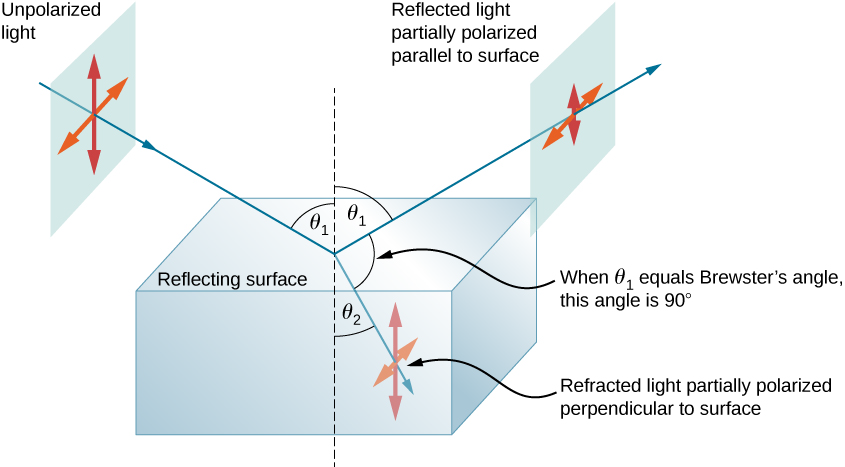
\includegraphics[width=.8\linewidth]{figures/polarization/reflaction.png}
    \caption{Polarization by reflection.
        \cite[Figure 1.38]{lingUniversityPhysicsVolume2016}}
    \label{fig:polarized_reflection}
\end{figure}

\subsection{Polarization Properties of Reflected Light}
When light reflects off a surface, its polarization changes \cite[34]{lingUniversityPhysicsVolume2016}.
This effect is illustrated in Figure \ref{fig:polarized_reflection} where the unpolarized light reflected off a surface becomes partially polarized.
Unpolarized light can be described as a sum of two orthogonal linear polarizations $R_\perp$ and $R_\parallel$, where $R_\perp$ is perpendicular to the plane of incidence and $R_\parallel$ is parallel to the plane of incidence.
These two components are referred to as s-polarized and p-polarized light, respectively, and their reflection coefficients are given by the Fresnel equations below:

\begin{align}
    R_\perp =     & \left|{\frac {n_{1}\cos \theta _1-n_{2}\cos \theta _2}{n_{1}\cos \theta _1+n_{2}\cos \theta _2}}\right|^{2}
                  & 
    R_\parallel = & \left|{\frac {n_{1}\cos \theta _2-n_{2}\cos \theta _1}{n_{1}\cos \theta _2+n_{2}\cos \theta _1}}\right|^{2}
\end{align}

Where  $\eta_1$ and $\eta_2$ are the refractive indices of the two media,
$\theta_i$ is the angle of incidence and $\theta_r$ is the angle of refraction.
Using the trigonometric identity $ \cos^2{\left(\theta_2 \right)} = 1- \sin^2{\left(\theta_2 \right)}$ and Snell's law $\eta_1 \sin{\left(\theta_1 \right)} = \eta_2 \sin{\left(\theta_2 \right)}$ the angle of refraction, $\theta_2$ can be removed, and the equations can be rewritten as:

\begin{align}
    R_\perp =     & \left|{\frac {n_{1}\cos \theta _1-n_{2}{\sqrt {1-\left({\frac {n_{1}}{n_{2}}}\sin \theta _1\right)^{2}}}}{n_{1}\cos \theta _1+n_{2}{\sqrt {1-\left({\frac {n_{1}}{n_{2}}}\sin \theta _1\right)^{2}}}}}\right|^{2}
                  & 
    R_\parallel = & \left|{\frac {n_{1}{\sqrt {1-\left({\frac {n_{1}}{n_{2}}}\sin \theta _1\right)^{2}}}-n_{2}\cos \theta _1}{n_{1}{\sqrt {1-\left({\frac {n_{1}}{n_{2}}}\sin \theta _1\right)^{2}}}+n_{2}\cos \theta _1}}\right|^{2}
\end{align}





Inserting the refractive index of air, $n_1 = 1$, and the refractive index of water, $n_2 = 1.33$, the reflectance can be calculated and plotted as a function of the angle of incidence, $\theta_1$, alone as shown in Figure \ref{fig:brewster0}.
The \gls{dolp} is the degree to which light is linearly polarized and can be defined as the ratio between the difference and the sum of the two polarization components.
The \gls{dolp} is plotted in Figure \ref{fig:brewster1}.
At one particular angle of incidence, $\theta_B$, known as the Brewster angle, $R_\parallel$ becomes zero, and the reflected light is completely s-polarized:
\begin{align}
    \theta_B & = \arctan{\frac{n_2}{n_1}} & DoLP= & \frac{\left | R_\perp - R_\parallel \right |}{R_\perp + R_\parallel}
\end{align}

\begin{figure}[H]
    \centering
    \begin{subfigure}{.5\textwidth}
        \centering
        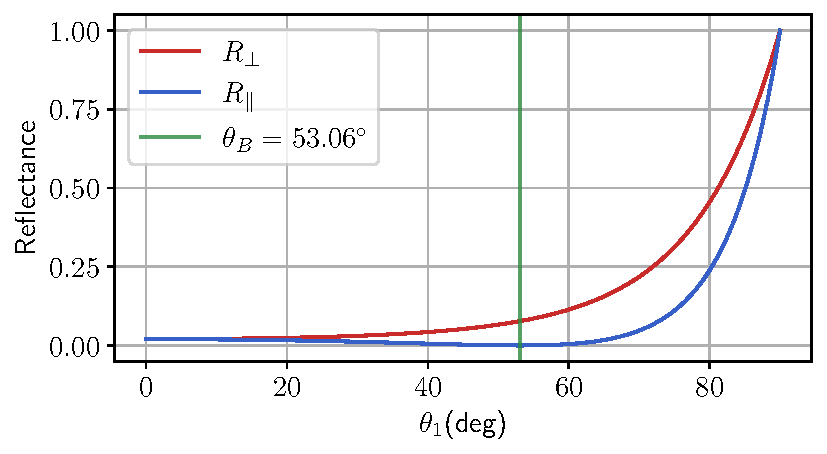
\includegraphics[width=\textwidth]{figures/pol_plots/brewster0.pdf}
        \caption{Reflectance of S and P polarized light of water.}
        \label{fig:brewster0}
    \end{subfigure}%
    \begin{subfigure}{.5\textwidth}
        \centering
        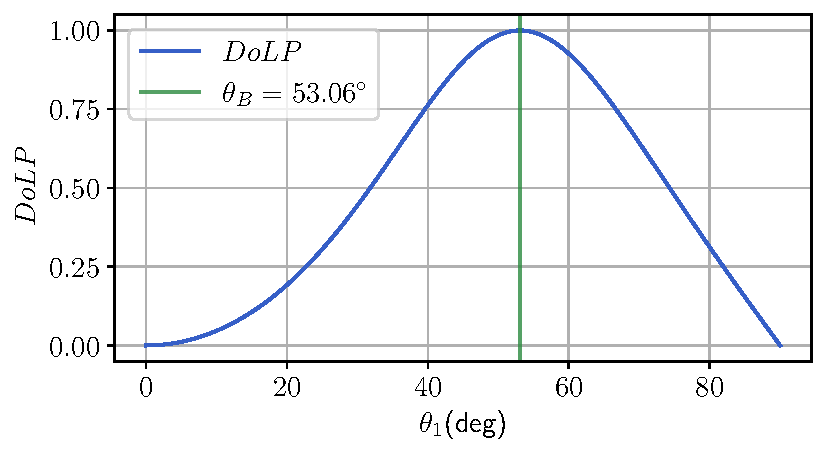
\includegraphics[width=\textwidth]{figures/pol_plots/brewster1.pdf}
        \caption{\gls{dolp} of light reflected off water. \label{fig:dolp_graph}}
        \label{fig:brewster1}
    \end{subfigure}
    \caption{Reflectance and \gls{dolp} of light reflected off water as a function of the angle of incidence.
        The Brewster angle is marked with a vertical line.}
    \label{fig:test}
\end{figure}




\subsection{Estimating Polarization Properties of Light using Polarizers}
In polarized light, the electromagnetic oscillations trace an elliptical path, which simplifies to a circular or straight line for pure circular or linear polarization, respectively.
When light passes through a linear polarizer, the electric field is filtered, allowing only the component aligned with the polarizer to continue through.
By aligning four linear polarizers at 45-degree intervals, the \glsfirst{dolp} and \glsfirst{aolp} can be determined as shown in Figure \ref{fig:polarization_calculation}.

\begin{figure}[H]
    
    \begin{minipage}{.48\textwidth}
        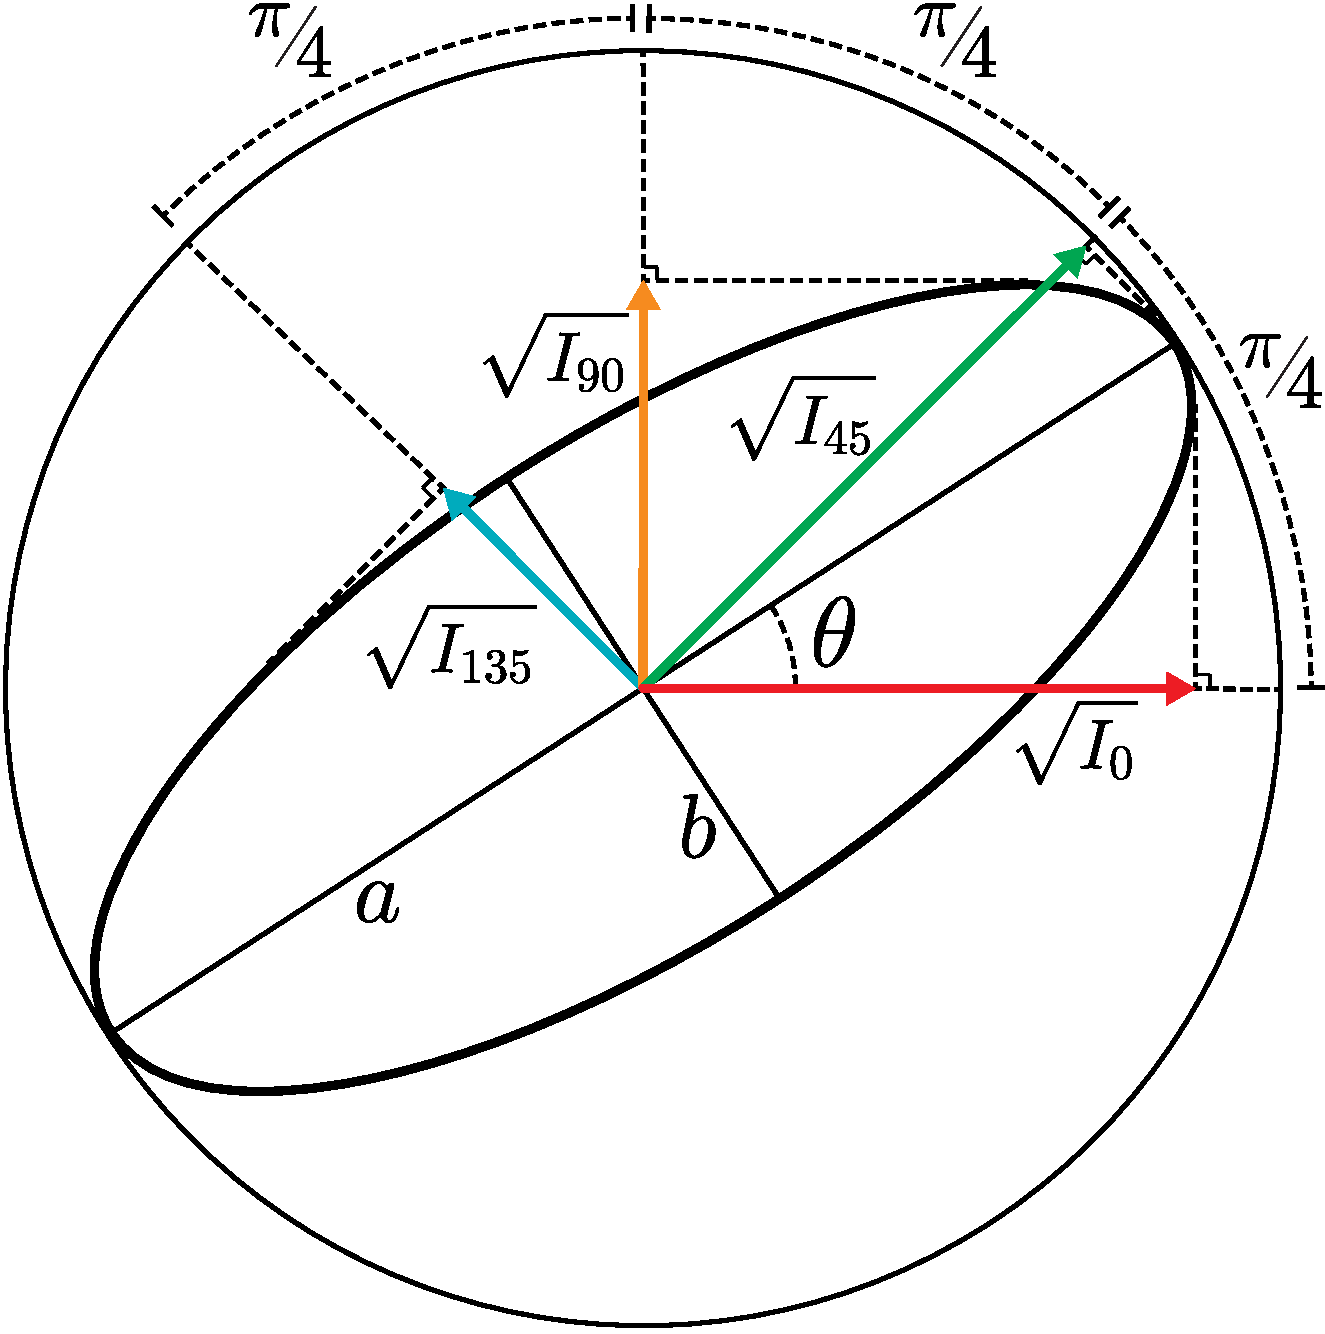
\includegraphics[width=\textwidth]{figures/polarization_sketch.pdf}
    \end{minipage}
    \hfill
    \begin{minipage}{.48\textwidth}
        \begin{alignat}{3}
             & \mathrlap{\cos\theta \cdot a\cos t -  \sin\theta \cdot b\sin t}                & 
             &                                                                                & 
             &                                                                                   \\
             &                                                                                & 
             & = \mathrlap{\sqrt{a^2\cos^2\theta+b^2\sin^2\theta} \cos(\omega + \phi)}        & 
             &                                                                                   \\[1em]
             & I_0                                                                            & 
             & = \mathrlap{a^2\cos^2\theta + b^2\sin^2\theta                                } & 
             &                                                                                   \\
             & I_{45}                                                                         & 
             & = \mathrlap{a^2\cos^2(\theta-\frac{\pi}{4}) + b^2\sin^2(\theta-\frac{\pi}{4})} & 
             &                                                                                   \\
             & I_{90}                                                                         & 
             & = \mathrlap{a^2\sin^2\theta + b^2\cos^2\theta                                } & 
             &                                                                                   \\
             & I_{135}                                                                        & 
             & = \mathrlap{a^2\sin^2(\theta-\frac{\pi}{4}) + b^2\cos^2(\theta-\frac{\pi}{4})} & 
             &                                                                                   \\[1em]
             & S_0                                                                            & 
             & = I_0 + I_{90}                                                                 & 
             & = a^2+b^2                                                                         \\
             & S_1                                                                            & 
             & = I_0 - I_{90}                                                                 & 
             & =(a^2-b^2)\cos(2x)                                                                \\
             & S_2                                                                            & 
             & = I_{45} - I_{135}                                                             & 
             & =(a^2-b^2)\sin(2x)                                                                \\[1em]
             & DoLP                                                                           & 
             & =\frac{a^2-b^2}{a^2+b^2}                                                       & 
             & = \frac{\sqrt{S_1^2 + S_2^2}}{S_0}                                                \\
             & AoLP                                                                           & 
             & =  \theta                                                                      & 
             & = \frac{1}{2}\arctan{\left(\frac{S_2}{S_1}\right)}
        \end{alignat}
    \end{minipage}%
    
    \caption{How four linear polarizers placed at $45^\circ$ intervals can be used to calculate the \gls{dolp} and \gls{aolp} of polarized light. \label{fig:polarization_calculation}}
\end{figure}%

\section{Polarization Cameras}
The sensor rig is equipped with two TRI050S1-QC cameras from Lucid Vision Labs.
The cameras use a 5MP \gls{cpfa} sensor from Sony capable of capturing both color and polarization information. 
In this sensor every pixel is equipped with a color filter and a polarization filter, as shown in Figure \ref{fig:cpfa}.

\begin{figure}[H]
    \begin{subfigure}[B]{.48\textwidth}
        \centering
        
\includegraphics[width=\textwidth]{figures/sensor_layout.pdf}
        \caption{\gls{cpfa}. The numbers represents the filter angles.\label{fig:cpfa}}
    \end{subfigure}
    \hfill
    \begin{subfigure}[B]{.48\textwidth}
        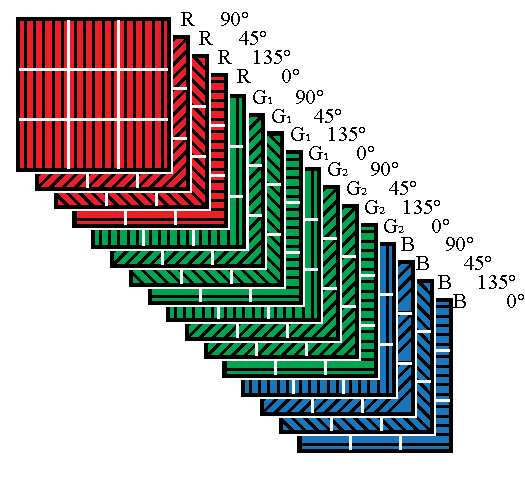
\includegraphics[width=\textwidth]{figures/sensor_packaging.pdf}
        \caption{Reordered view of \ref{fig:cpfa}. \label{fig:cpfa_reorder}}
    \end{subfigure}
    \caption{A 12\times12 slice of the \gls{cpfa} used in TRI050S1-QC cameras \cite{lucidvisionlabsTritonMPPolarized2020}, and how the the data can be reorderd as a 3\times3 image with 16 channels. \label{fig:polarization_sensor}}
\end{figure}%

% \subsection{A Simple Color-Polarization Demosaicking Approach}
\pagebreak
Similar to how debayering is used to estimate the missing color channels from a Bayer filter, color-polarization demosaicking is used to estimate the missing polarization channels from a \gls{cpfa} sensor.
With the physical displacement of the filters on the sensors it's important to compensate for gradients in the scene to avoid aliasing artifacts.
Several methods that solve this and perform accurate color-polarization demosaicking exist, but we propose a simple linear method that can be implemented with a single convolutional layer \cite{morimatsuMonochromeColorPolarization2020}\cite{morimatsuMonochromeColorPolarization2021}\cite{nguyenTwoStepColorPolarizationDemosaicking2022a}.
The method estimates $S0$, $S1$, and $S2$ for each color channel at every pixel, i.e. it transforms the $n \times m \times 1$ raw \gls{cpfa} image into a $n \times m \times 9$ image.

First, the raw \gls{cpfa} input image is permuted into a $(n/4) \times (m/4) \times 16$ image, where the 16 channels correspond to the different color and polarization filters as depicted in Figure \ref{fig:cpfa_reorder}.
A custom CUDA kernel was written to unpack raw camera data and perform this permutation in one step, but the same result can be achieved with the following tensor operations using a library like PyTorch:
\begin{figure}[H]
    \centering
    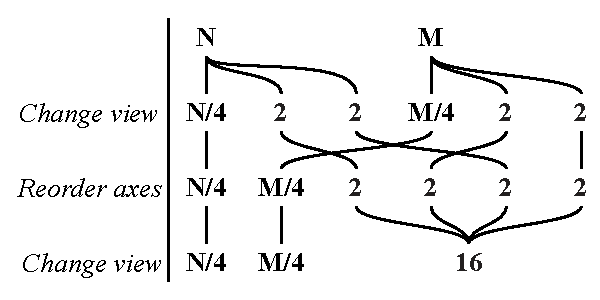
\includegraphics[width=.6\textwidth]{figures/transformation.pdf}
    \caption{Permutations from a $n \times m \times C $ tensor to a $(n/4) \times (m/4) \times (C\times 16)$ tensor. \label{fig:reorder_operations}}
    
\end{figure}%

Then, a single convolutional layer is applied to obtain a $(n/4)*(m/4)*144$ image.
Finally, the image is permuted back to a $n \times m \times 9$ image by reversing the operations in Figure \ref{fig:reorder_operations}.
With a kernel size of 5, the convolutional layer has only $144\times16\times5\times5=57600$ weights.
Since we only use a single convolution operation, the transformation is linear, and we can find the least square solution directly without the use of gradient descent.
The weights were fitted to the Tokyo Tech dataset, a 12-channel (3 colors \times 4 angles) color-polarization image dataset with 40 scenes \cite{morimatsuMonochromeColorPolarization2020}\cite{morimatsuMonochromeColorPolarization2021}.
To simulate raw \gls{cpfa} images, we select the channel for each pixel with the same color and polarization angle as the corresponding pixel in the \gls{cpfa} image.
Figure \ref{fig:cpfa_demosaicking} shows how this method is used to obtain and visualize the polarization information from a \gls{cpfa} image.

To increase the size of the dataset, we used all 16 possible placements of the virtual \gls{cpfa} on each image by shifting the images up to 3 pixels in each direction.
We also augmented the dataset by flipping the images horizontally and vertically.


\begin{figure}[H]
    \begin{subfigure}[T]{.49\textwidth}
        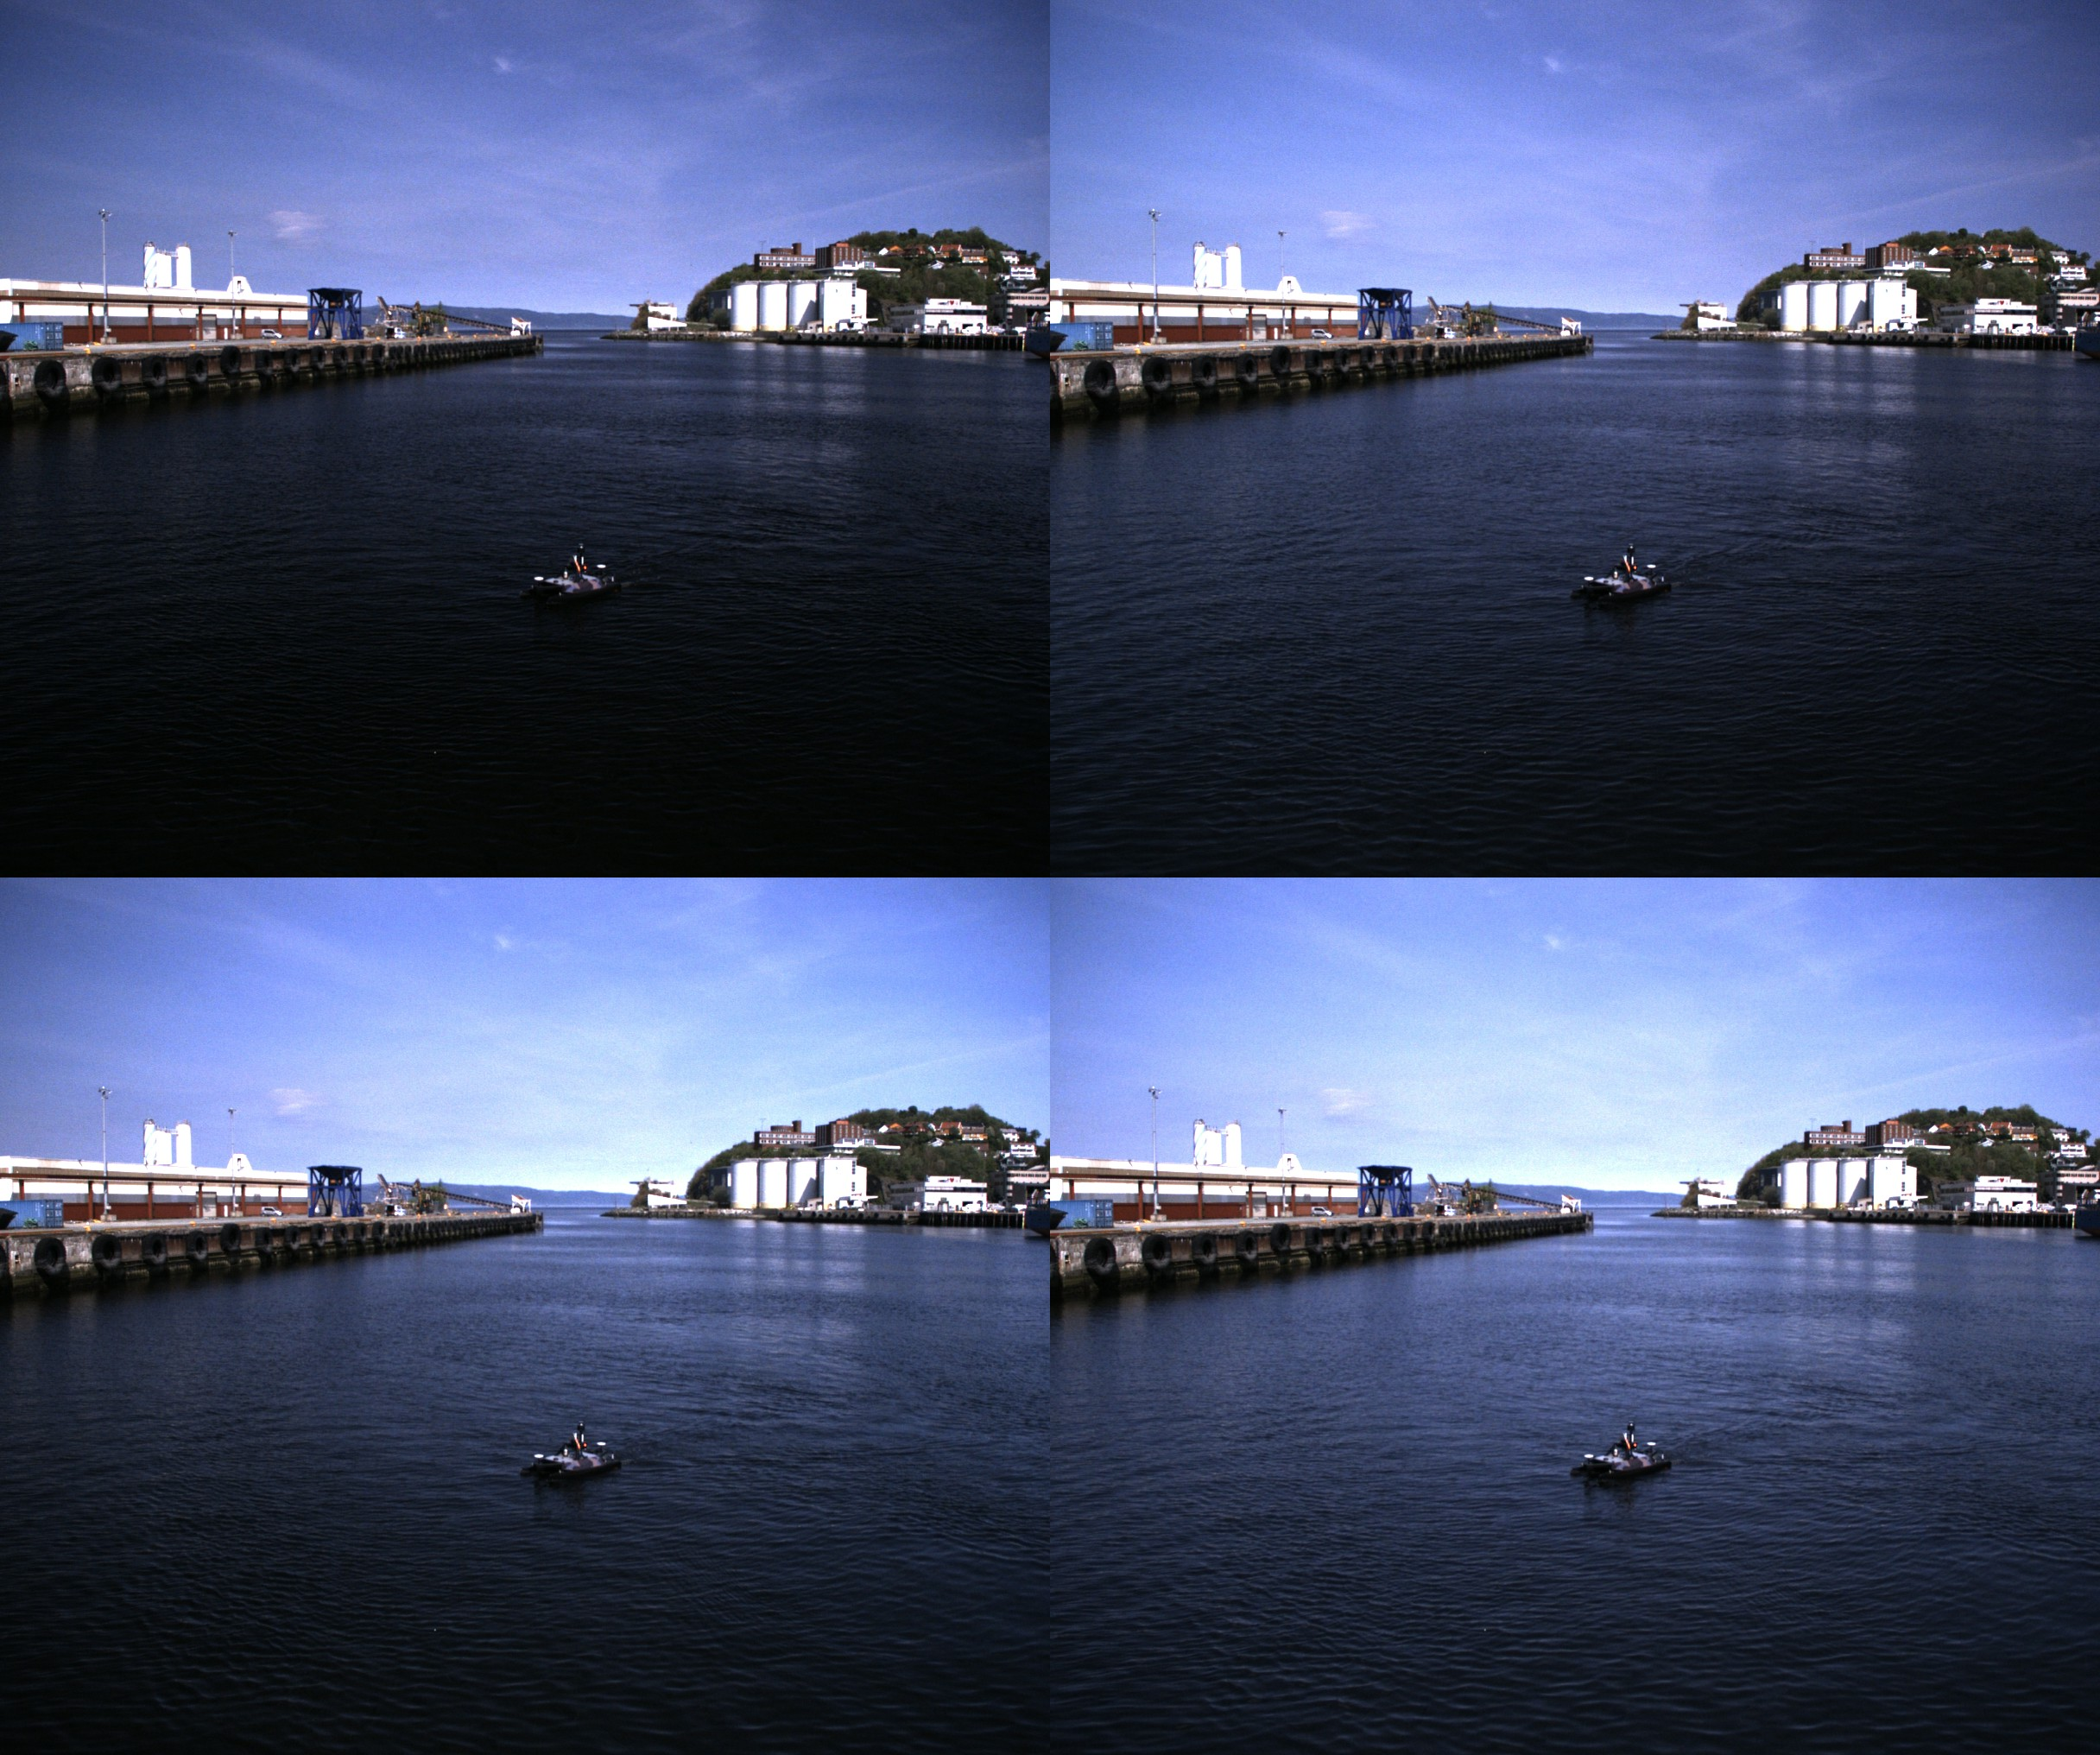
\includegraphics[width=\textwidth]{figures/img_0080_right_inten.jpg}
        \caption{$I90$, $I45$, $I135$, and $I0$.}
    \end{subfigure}
    \hfill
    \begin{subfigure}[T]{.49\textwidth}
        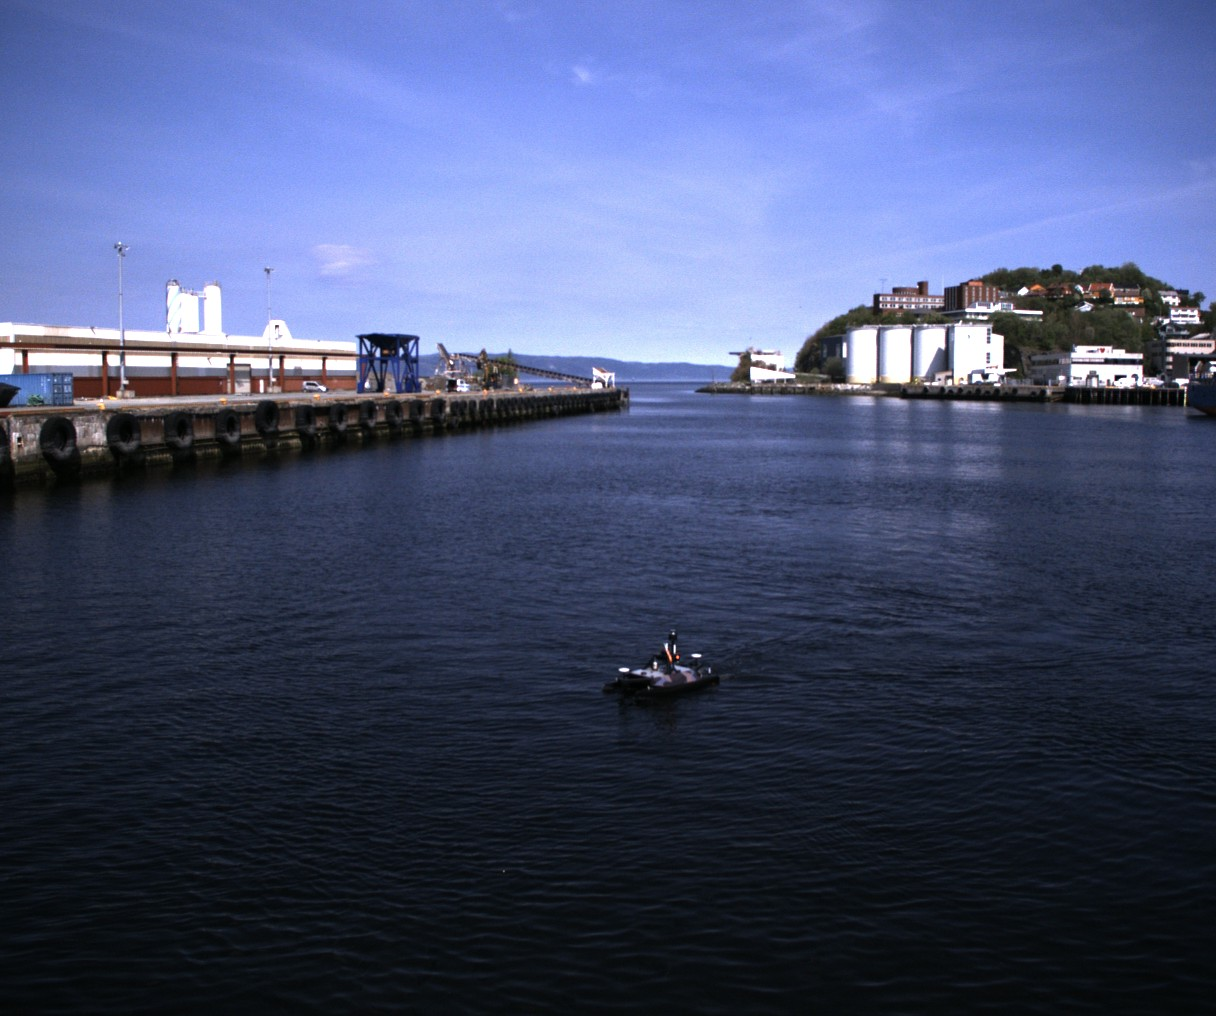
\includegraphics[width=\textwidth]{figures/img_0080_right_s0.jpg}
        \caption{$S_0$, equivalent to what a normal camera would capture.}
    \end{subfigure}
\end{figure}

\begin{figure}[H]\ContinuedFloat
    \begin{subfigure}[B]{.49\textwidth}
        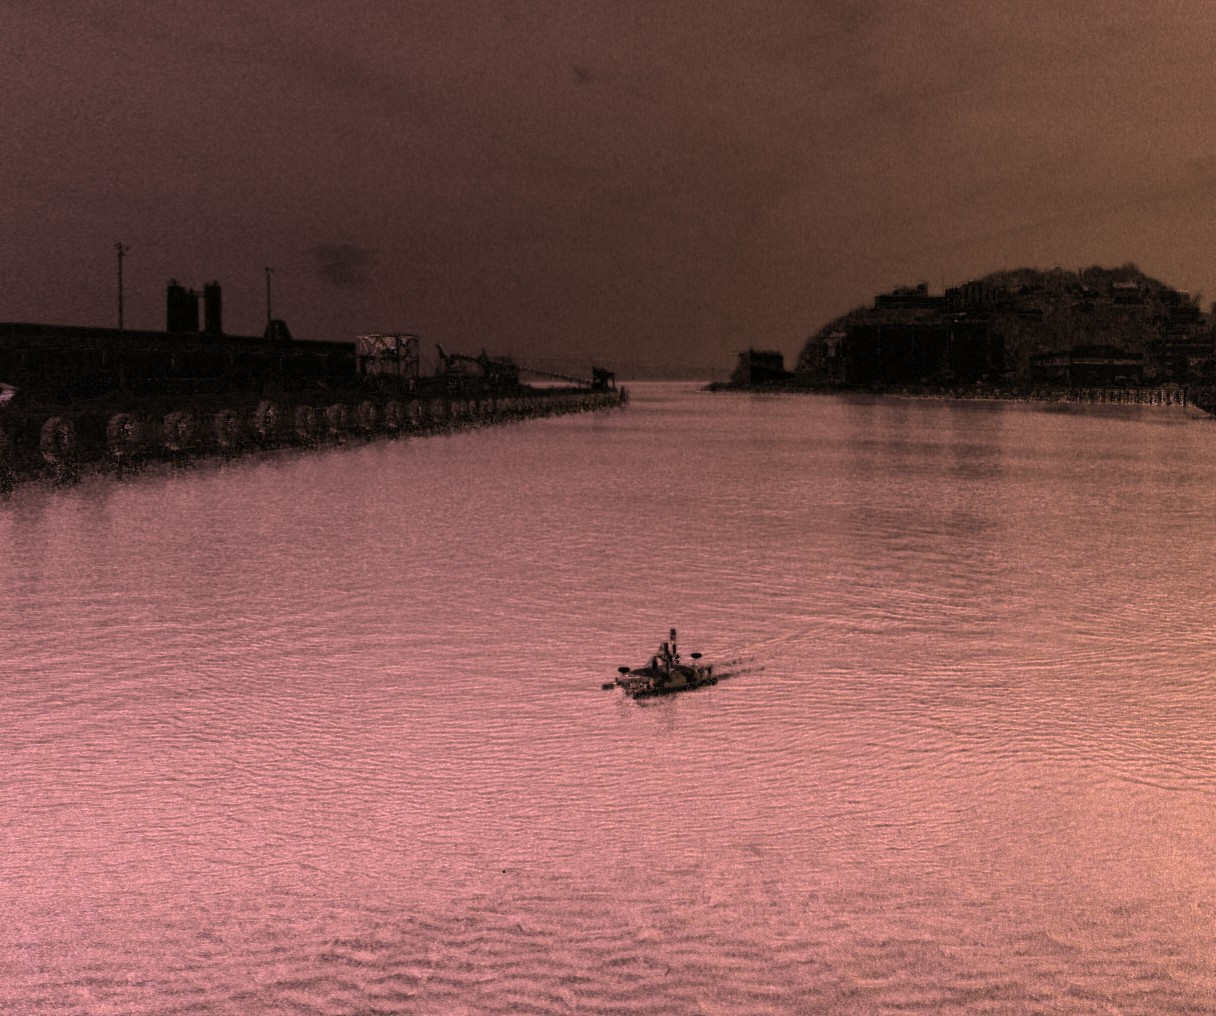
\includegraphics[width=\textwidth]{figures/img_0080_right_pol.jpg}
        \caption{Visualization of \gls{dolp} and \gls{aolp} for luminance. Similar visualizations can be made for each separate color channel.}
    \end{subfigure}
    \hfill
    \begin{subfigure}[B]{.49\textwidth}
        \centering
        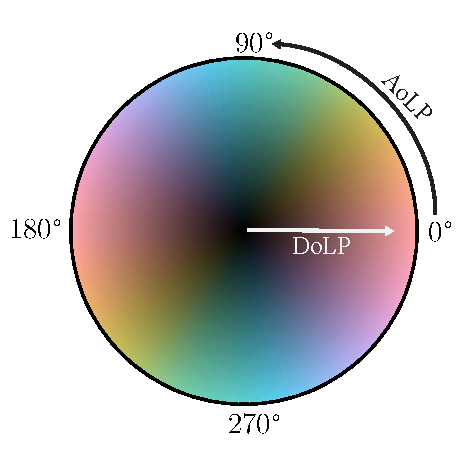
\includegraphics[width=.8\textwidth]{figures/cmap/aolp_dolp_cmap.pdf}
        \vspace{1em}
        \caption{Colormap used to visualize \gls{dolp} and \gls{aolp}. Using a colormap with constant luminance, rather than HSV, makes it easier to visually determine \gls{dolp}. }
    \end{subfigure}
    \caption{An image captured with a color polarization filter array sensor and visualization of its polarization information. \label{fig:cpfa_demosaicking}}
\end{figure}

% \hfill



% \section{Debayering of Color Polarization Images}

% \begin{align*}
%     \text{BT709} = \begin{bmatrix}
%                        0.2126  & 0.7152  & 0.0722  \\
%                        -0.1146 & -0.3854 & 0.5     \\
%                        0.5     & -0.4542 & -0.0458
%                    \end{bmatrix}
% \end{align*}



\section{Sensor Rig Design}
The sensor rig is designed to carried and operated by a single person, but can also be attached to a vessel.
Two 1m carbon fiber tubes servs as the main structure and provides rigidity to the rig without adding much weight.
Except for the waterproof enclosure and the two carbon fiber tubes, all the mechanical parts are 3D printed, making the sensor rig easy to reproduce and modify.
The various parts are designed to clamp on to the 30mm carbon fiber tubes and friction tape is used to ensure a tight fit.
This makes it easy to extend the rig with additional sensors or design various clamping brackets for attaching the rig to different vessels.
An IP67 rated waterproof enclosure is used to protect the internal electronics from the elements, allowing for operation in different weather conditions.
The components inside the enclosure are mounted on two detatchable 3D printed plates that are locket in place by a wedge system, making it easy to remove and replace the components if neded.
Both the wieght and cost of the sensor rig is dominated by the coice of components, which can be adjusted to fit the needs of the user.

\begin{figure}[H]
    \centering
    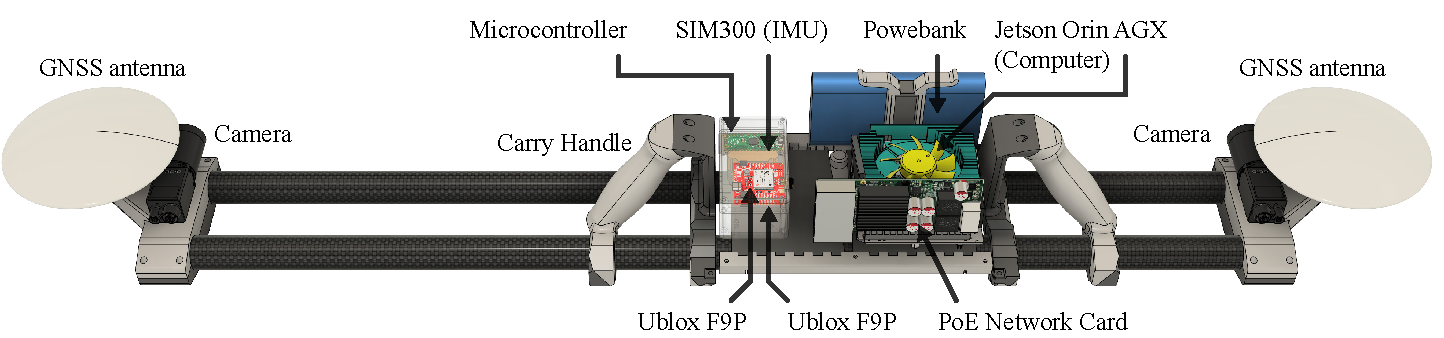
\includegraphics[width=\textwidth]{figures/rig_components.pdf}
    \caption{Cad model of the sensor rig with the enclosure removed for visibility.}
\end{figure}

\subsection{Components}
In its current configuration, one TRI050S1-QC polarization camera and one TOP106 L1/L2 GNSS antenna is mounted on each side of the sensor rig to provide wide baseline stereo video and differential GNSS data for accurate heading estimation.
The cameras have a 2/3" global shutter sensor with a $2448\times2048$ resolution, are equipped with a 8mm lense, and configured to capture 12-bit raw images at 12fps.
Inside the waterproof enclosure an Nvidia Jetson Orin AGX serves as the main processing unit.
The Jetson is a single board computer designed for edge computing with a dedicated GPU, GPIO and multiple dedicated hardware for video processing and AI \cite{karumbunathanNVIDIAJetsonAGX2022}.
An external network card is connected to the Jetson through its PCIe slot and provedes 4 separate 1Gb/s ethernet ports with \gls{poe} to power and communicate with the cameras over a single cable.
Two F9P GNSS receivers and a STIM300 \gls{imu} provide the sensor data required for accurate pose estimation.
With a 100wh detatchable power bank, the sensor rig can record data for approximately 5 hours before needing a battery change.

\begin{figure}[H]
    \centering
    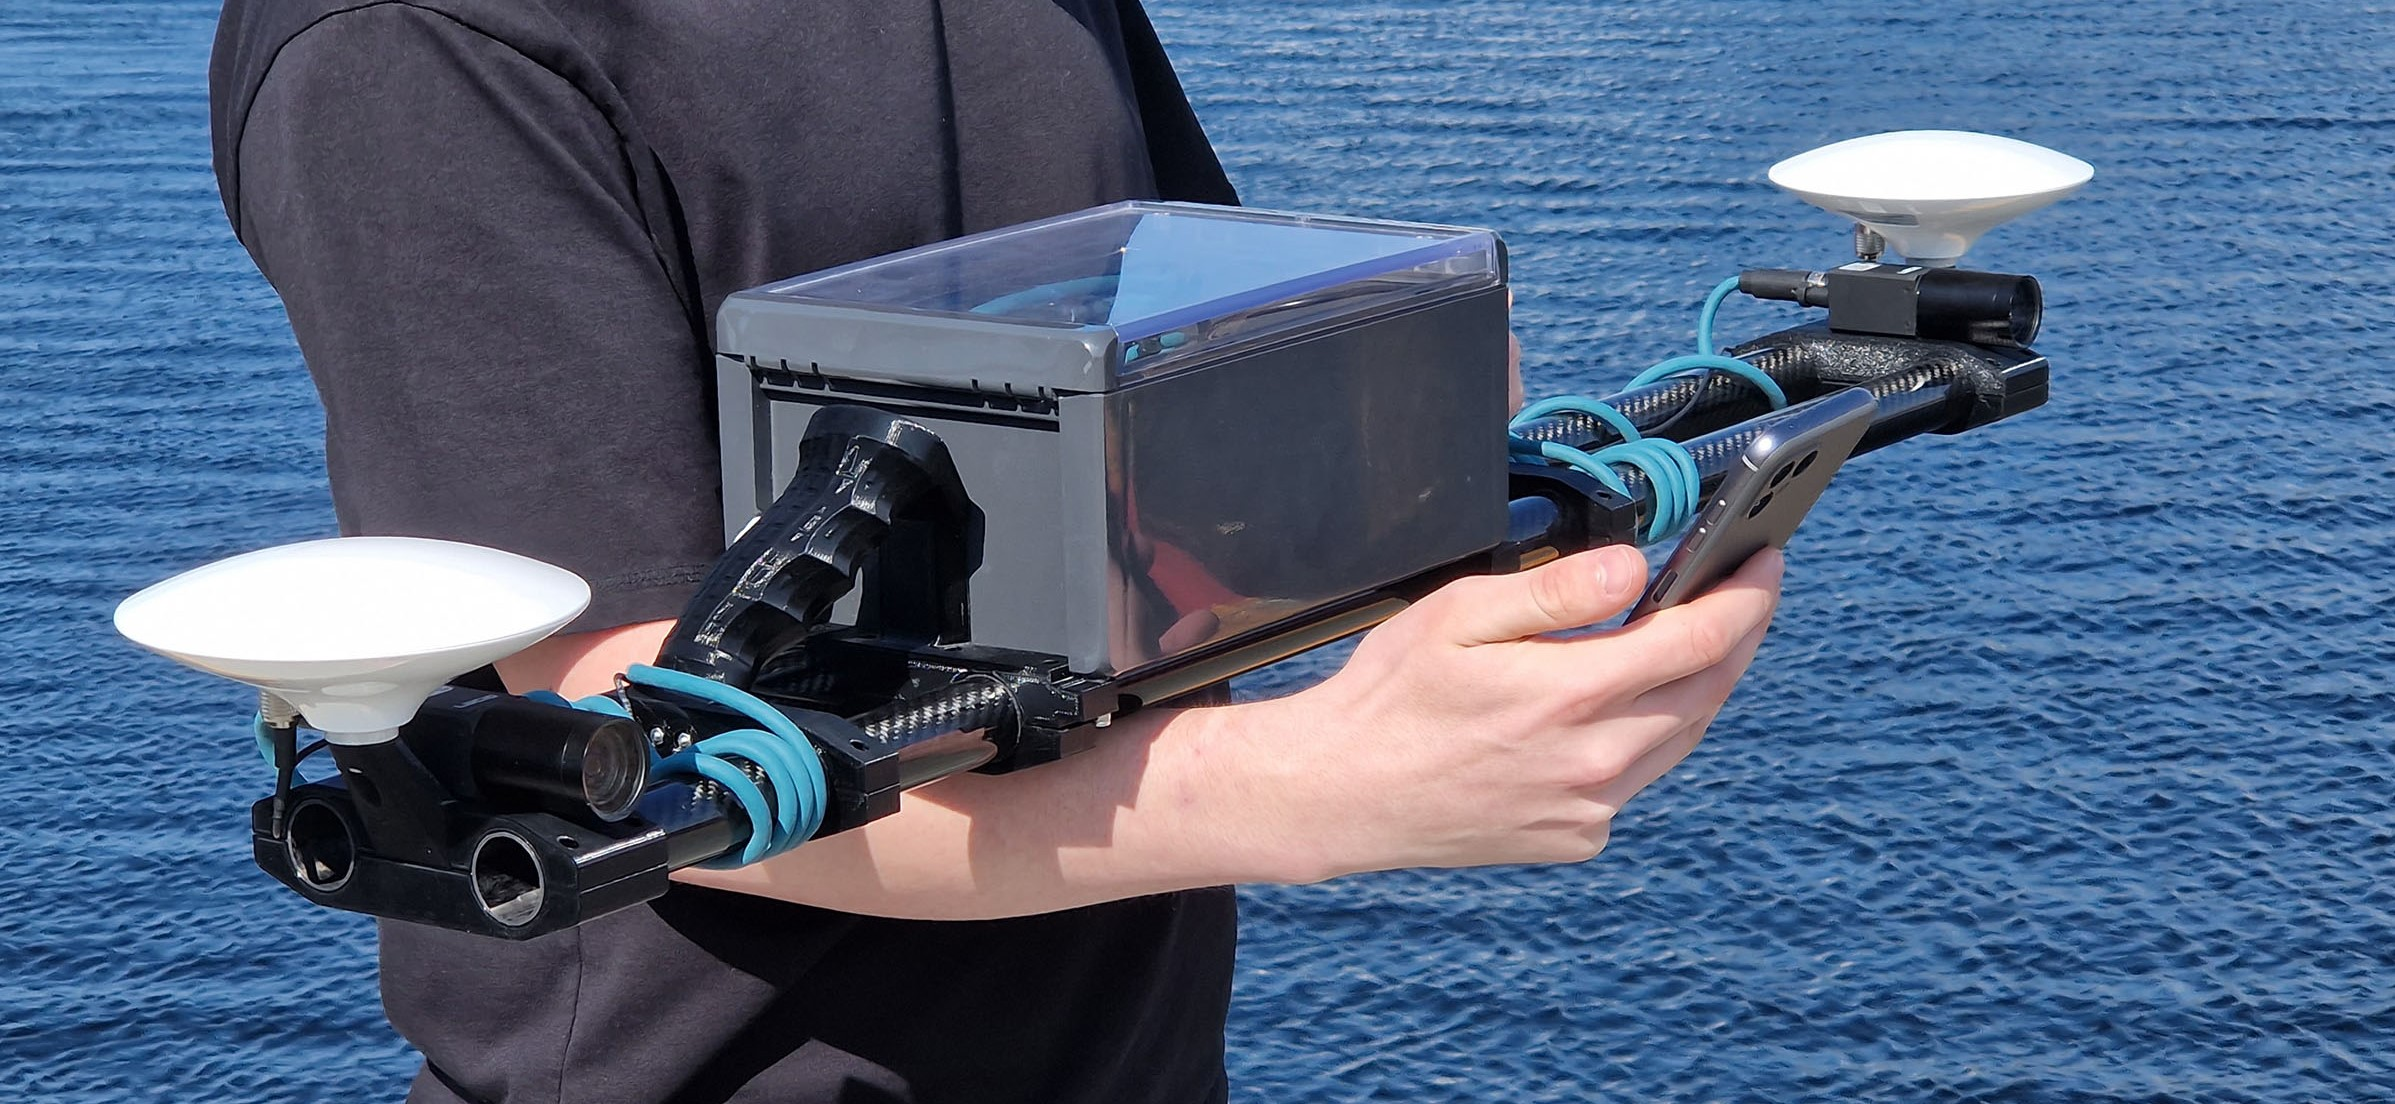
\includegraphics[width=\textwidth]{figures/operation.jpg}
    \caption{Human operation of the sensor rig. Ergonomic handles ensure comfort and the operator can control and monitor the acquisition through a phone over the phone's mobile hotspot. \label{fig:operation}}
\end{figure}

\subsection{Control and Monitoring}
The sensor rig hosts a web app that allows the operator to control and monitor the data acquisition from their smartphone, as depicted in Figure \ref{fig:operation}.
The web app is built with SvelteKit and communicates with the different programs running on the Jetson through websockets.
From the app the operator can start and stop the aquisition, incoming data from the different sensors and view a live stream from the cameras.
The app also provides information from the Jetson such as CPU temperature, storage usage, \gls{pps} status and battery voltage.
Earlier versions of the app alowed the user to configure parameters such as exposure and gain but we noticed that this took away focus so we swithed to automatic adjustment of these parameters.
Having a simple interface makes it possible for almost anyone to use the sensor rig and adds to its usability.


\subsection{Synchronization}
Emphasis has been put on accurately synchronizing all sensors on the sensor rig to \gls{utc}.
The \gls{gnss} receivers are synchronized to \gls{utc} by them selves, and does not require further synchronization.
The \gls{imu} samples at a fixed frequency following an internal clock \cite{safranSTIM300Datasheet}.
When it receives a trigger signal it sends the latest available data, together with the trigger count and the delay between the latest message and the trigger \cite{safranSTIM300Datasheet}.
To synchronize the \gls{imu} to \gls{utc} we use a Raspberry Pi Pico microcontroller to periodically route the trigger signal to the \gls{imu} and the \gls{f9p} receiver simultaneously, causing the \gls{f9p} to log a time mark message we use to stamp the \gls{imu} data \cite[190]{u-bloxZEDF9PInterfaceDescription}.
The cameras and the network card all support \gls{ptp}, making it possible to synchronize the cameras to the clock on the Jetson.
Using an oscilloscope we measured the synchronization error between the cameras to be below $20\mu s$ by comparing the trigger signal emitted from the cameras.
The final step in the syndhronization process is to synchronize the Jetson to \gls{utc} using the \gls{pps} signal from one of the \gls{f9p} receivers.
This requiered making several modification to, and compiling, the linux kernel running on the Jetson, which took considerable time and effort.
A script that downloads, modifies and compiles all the necessary files is available on request.
The reported accuracy of the \gls{pps} synchronization is reported to be approximately $4\mu s$.








\section*{Synchronization}

\subsection*{Computer}
Compiling Linux Kernel


\subsection*{IMU}
Microcontroller send interrupt to F9P and log TM2 messages.
Variable frequency to ensure synchronization if messages are lost.

\subsection*{Cameras}
Use cameras and network card that support PTP.


\begin{figure}[H]
    \centering
    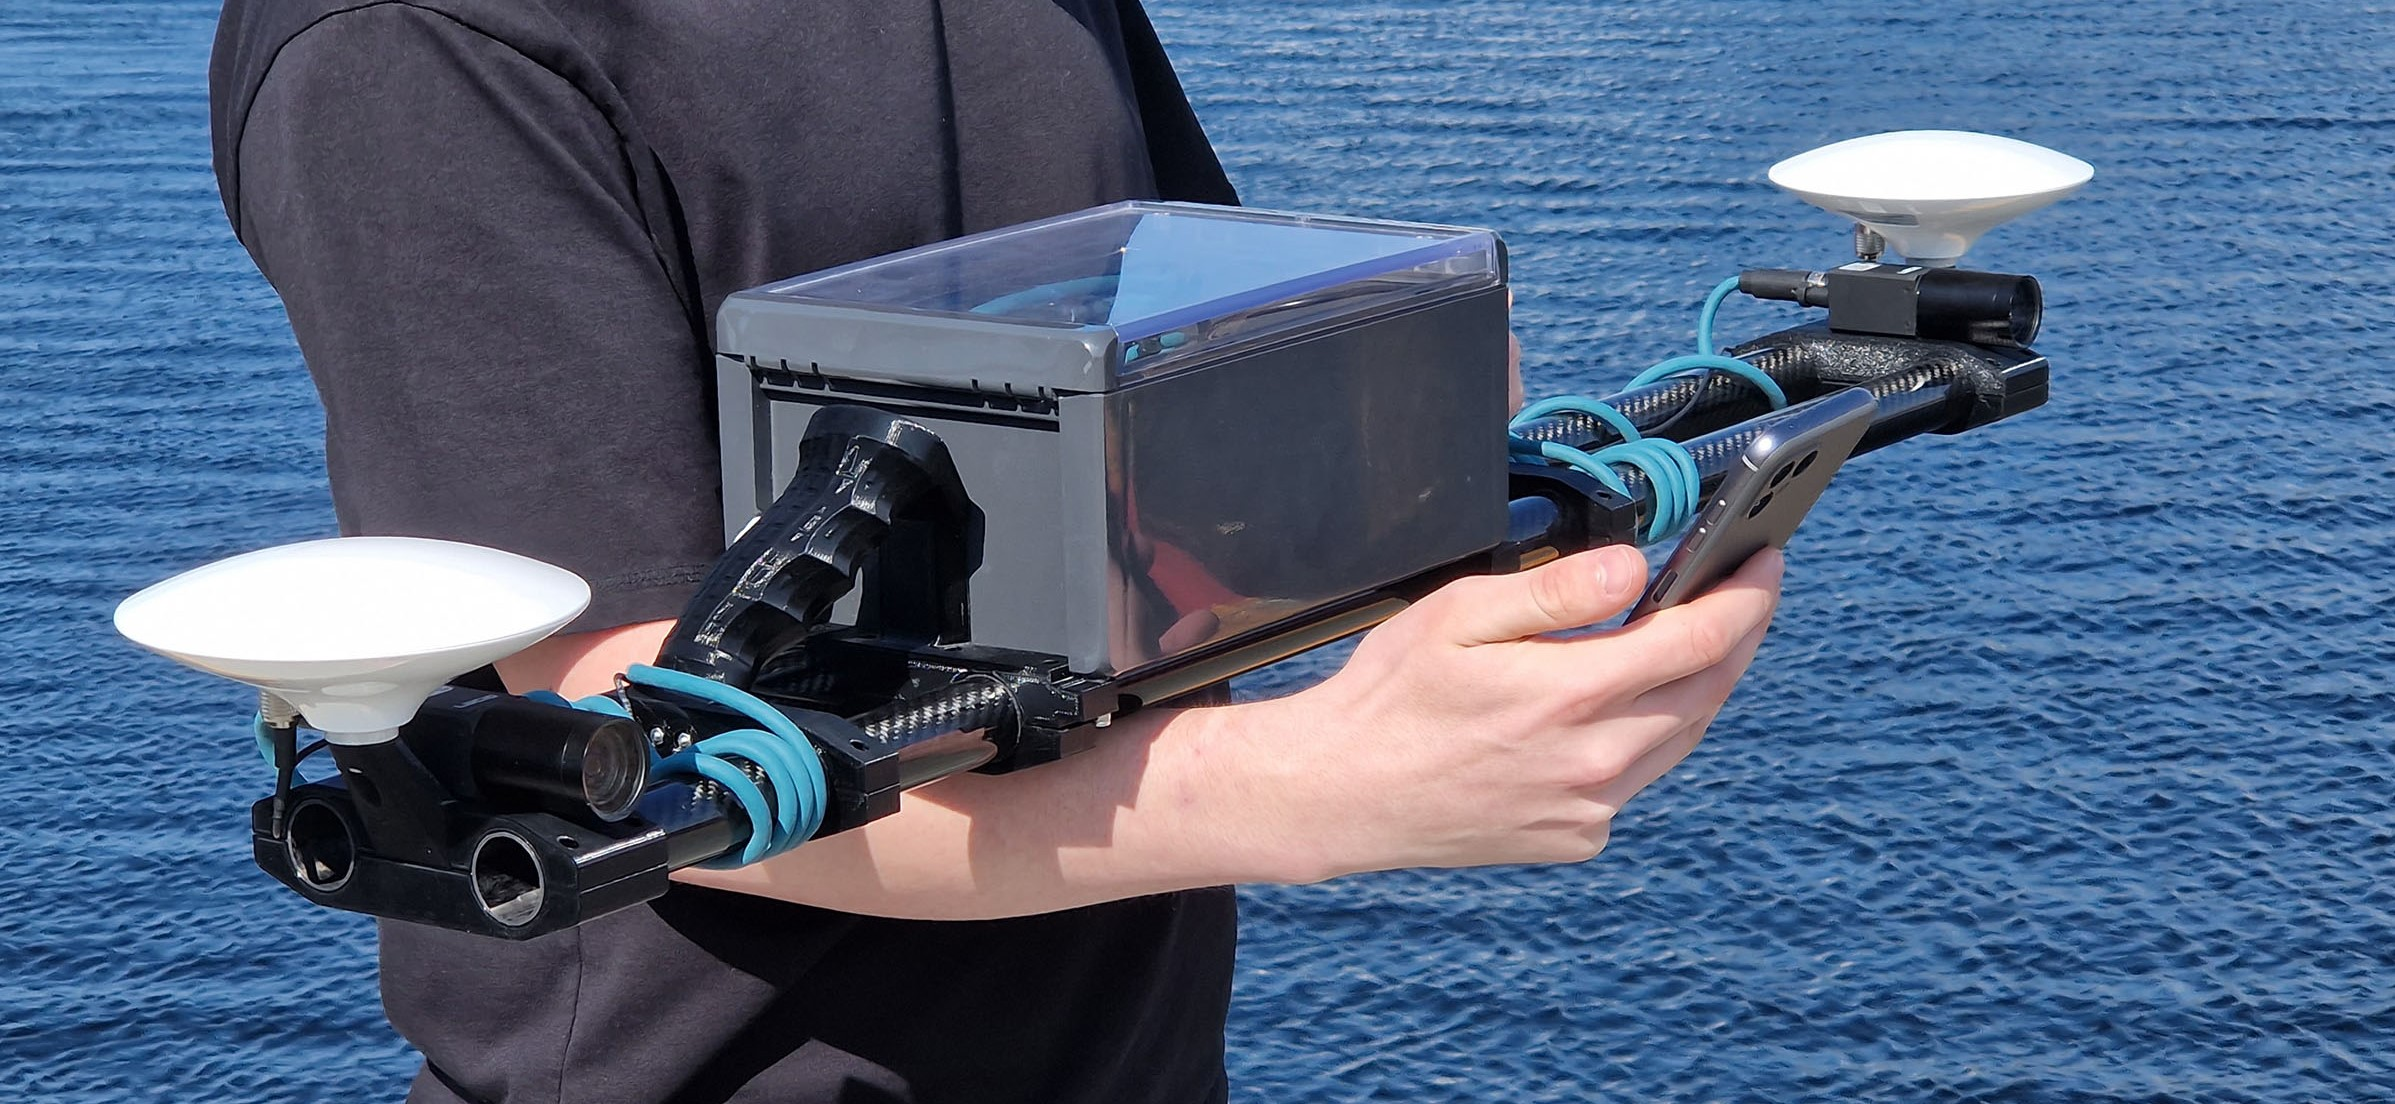
\includegraphics[width=\textwidth]{figures/operation.jpg}
    \caption{Human operation of the sensor rig. Ergonomic handles ensure comfort and the operator can control and monitor the acquisition through a phone over the phone's mobile hotspot.}
\end{figure}

% \printglossary[type=\acronymtype]
\printglossary

\printbibliography


\end{document}